\documentclass[10pt, a4paper, twocolumn]{article}

\usepackage{stage}

\bibliography{biblio}

% Set stuff for title
\title{Shape-Adaptive Kernel Density Estimation}
\author{L.E.N. Baakman}

\begin{document}

\twocolumn[
  \begin{@twocolumnfalse}
    \maketitle
		\begin{abstract}
			%!TEX root = paper.tex
% Introduction
\noindent Kernel density estimation is a popular method to approximate probability densities in numerous fields.
% Method
Generally these methods use symmetric kernels, even though the data of which the density is estimated are not necessarily spread equally in all dimensions. To account for this asymmetric distribution of data we propose the use of shape adaptive kernels: kernels whose shape changes to fit the spread of the data in the local neighborhood.
% Experiment
We compare the performance of the shape adaptive kernels with that of an estimator that uses a symmetric kernel on simulated datasets with known density fields.
% Results
No significant differences in performance between the symmetric and the shape-adaptive estimator were found. Although the former outperformed the latter on points near the boundary of the datasets. We also found some differences in performance dependent on the distance to the mean of Gaussian distributions with low values on the diagonal of the covariance matrix.  
% Conclusion
In conclusion shape-adaptive kernels are a promising idea that warrants further research.

		\end{abstract}
		\vspace{2em}
  \end{@twocolumnfalse}
]

\section{Introduction}
\label{s:introduction}
%!TEX root = paper.tex
Estimating densities with kernels has been fairly popular of late; in the medical field it has been used to predict dose-volume histograms, which are instrumental in the determination of radiation doses \cite{SkarpmanDose2015}. Ecologists have applied it to explore the habitats of seabirds \cite{lees2016using}. \textcite{ferdosi2011comparison} have described it as ``a critical first step in making progress in many areas of astronomy."  Within this discipline  density estimation is, among other things, used to estimate the density of the cosmic density field, which is required for the reconstruction of the large-scale structure of the universe.

Formally the aim of density estimation is to find the probability density \varDensityFunction{\varPattern} in the \varDim-dimensional Euclidean space underlying \varNumPatterns points $\varPattern[1], \dotsc, \varPattern[\varNumPatterns]$, that have been selected independently from \varDensityFunction{\varPattern}. 

Kernel density estimation methods approximate \varDensityFunction{\varPattern} by placing bumps, referred to as kernels, on the different observations and summing these bumps to arrive at a final density estimate. This paper is concerned with a method to make the shape of these bumps adaptive to the local neighborhood of \varPattern. Before introducing the process used to determine the shape of the kernel we first review the different symmetric kernel density estimation methods that our approach is based on. 

% Parzen
	The Parzen approach \cite{parzen1962estimation} is one of the most simple kernel density estimation methods. It estimates the density of \varPattern according to:
	\begin{equation}\label{eq:1:parzen}
		\varEstimatedDensityFunction{\varPattern} = \frac{1}{\varNumPatterns}\sum_{\itXis = 1}^{\varNumPatterns} \varBandwidth^{-\varDim}\varKernel{\frac{\varPattern - \varPattern[\itXis]}{\varBandwidth}}.
	\end{equation}
	The shape of the bumps is determined by the kernel function \varKernel{\bullet}, its width by the bandwidth \varBandwidth. The Parzen approach requires the kernel to be a probability density function, \ie $\varKernel{\varPattern} \geq 0$ and $\int \varKernel{\varPattern} = 1$ \cite{silverman1986density}. 
	%
	The bandwidth directly influences the result of the density estimation process; a too small bandwidth results in a density estimate with spurious fine structures, whereas kernels that are too wide can oversmooth the density estimate. Kernel estimators, such as the Parzen approach, that use kernels of the same width for all \varPattern[j], are called fixed-width estimators.

% Breiman, Meisel, Purcell
	One downside of fixed-width methods is that they cannot respond appropriately to variations in the magnitude of the density function, \ie the peakedness of the kernel is not data-responsive. Consequently in low density regions the density estimate will have peaks at the few sample points and be too low elsewhere. In areas with high density, the sample points are more densely packed together, which causes the Parzen estimate to spread out \cite{breiman1977variable}. Adaptive-width methods address this disadvantage of the fixed-width methods by allowing the width of the kernel to vary per data point. For example the estimator introduced by \citeauthor{breiman1977variable} uses the distance between \varPattern[\itXis] and the \KNNK-nearest neighbor of \varPattern[\itXis], denoted by \varKNNDistance{\itXis}{\KNNK}, to adapt the width of the kernel:
	%
	\begin{equation}\label{eq:1:BML}
	 	\varEstimatedDensityFunction{\varPattern} = \frac{1}{\varNumPatterns} \sum_{\itXis = 1}^{\varNumPatterns} (\varBMLconstant \cdot \varKNNDistance{\itXis}{k})^{-\varDim} \varKernel[\varGaussian]{\frac{\varPattern - \varPattern[\itXis]}{\varBMLconstant \cdot \varKNNDistance{\itXis}{k}}}.
	\end{equation} 
	%
	In \cref{eq:1:BML} \varKernel[\varGaussian]{} is used to represent a Gaussian kernel, and \varBMLconstant is a multiplicative constant. The values of both \varBMLconstant and \KNNK can be determined with a minimization algorithm on a goodness of fit statistic. Comparing \cref{eq:1:parzen} with \eqref{eq:1:BML} one finds that the bandwidth \varBandwidth of the Breiman estimator is defined as $\varBMLconstant\varKNNDistance{\itXis}{\KNNK}$. The second factor of this bandwidth depends on the local neighborhood of \varPattern[\itXis]. In low density regions \varKNNDistance{\itXis}{\KNNK} is large, and the kernel spreads out due to its high bandwidth. In areas with relatively many data points the converse occurs.

% Introduce Pilot Densities
	\textcite{silverman1986density} shows that the minimization procedure used by \citeauthor{breiman1977variable} implicitly uses a \KNN pilot estimate. If pilot estimates are used explicitly the density estimation process becomes:
		\begin{enumerate}[labelindent=0ex]
			\item \label{it:1:pilotdensities:pilotdensities}
				Compute pilot densities with some estimator that ensures that $\forall \itXis \; \varPilotDensityFunction{\varPattern[\itXis]} > 0$. 

			\item \label{it:1:pilotdensities:localbandwidths}
				Define local bandwidths $\varLocalBandwidth{i}$ as
				\begin{equation}\label{eq:1:localBandwidth}
					\varLocalBandwidth{\itXis} = \left( \frac{\varPilotDensityFunction{\varPattern[\itXis]}}{\varGeometricMeanFunction{\varPilotDensityFunction{\varPattern[0]}, \dotsc, \varPilotDensityFunction{\varPattern[\varNumPatterns]}}}  \right)^{- \varMBESensitivityParam},
				\end{equation}
				where $\varGeometricMeanFunction{}$ denotes the geometric mean and the sensitivity parameter \varMBESensitivityParam must lie in the range $\left[0, 1\right]$.
			\item \label{it:1:pilotdensities:finaldensities} 
				Compute the adaptive kernel estimate as
				\begin{equation}\label{eq:1:adaptiveKernelEstimateWithLocalBandwidths}
					\varEstimatedDensityFunction{\varPattern} = \frac{1}{\varNumPatterns} \sum_{\itXis = 1}^{\varNumPatterns} \left(\varBandwidth \cdot \varLocalBandwidth{\itXis}\right)^{-\varDim} \varKernel{\frac{\varPattern - \varPattern[\itXis]}{\varBandwidth \cdot  \varLocalBandwidth{\itXis}}}
				\end{equation}
				with \varKernel{} integrating to unity. 
		\end{enumerate}
	% Discuss step 1
	Since the pilot densities computed in step \ref{it:1:pilotdensities:pilotdensities} do not need to be sensitive to the fine details of the pilot estimate a convenient method, \eg the Parzen approach, can be used to estimate them \cite{silverman1986density}.
	% Discuss step 2
	The local bandwidths computed in \ref{it:1:pilotdensities:localbandwidths} depend on the exponent \varMBESensitivityParam. The higher this value is the more sensitive the local bandwidths are to variations in the pilot densities. Choosing $\varMBESensitivityParam = 0$ reduces \cref{eq:1:adaptiveKernelEstimateWithLocalBandwidths} to a fixed-width method.
		%Which value of \varMBESensitivityParam
		In the literature two values of \varMBESensitivityParam are prevalent. \citeauthor{breiman1977variable} argue that choosing $\varMBESensitivityParam = \rfrac{1}{\varDim}$ ensures that the number of observations covered by the kernel will be approximately the same in all areas of the data. Whereas \citeauthor{silverman1986density} favors $\varMBESensitivityParam = \rfrac{1}{2}$ independent of the dimension of the data, as this value results in a bias that can be shown to be of a smaller order than that of the fixed-width kernel estimate.
	% Discuss step 3

% Wilkinson and Meijer
	One disadvantage of the Breiman estimator is its computational complexity. This is partially due to the use of a Gaussian kernel. Because of the infinite base of this kernel an exponential function has to be evaluated \varNumPatterns times to estimate the density of one data point. 
	% First Change
	The Modified Breiman Estimator (MBE), introduced by \textcite{wilkinson1995dataplot}, reduces this computational complexity in two ways. Firstly they replace the infinite base Gaussian kernel with a spherical Epanechnikov kernel in both the computation of the pilot densities and the final density estimate. They define this kernel as:
	\begin{equation}\label{eq:1:epanechnikovKernelNoCovarianceMatrix}
		\varKernel[\varEpan]{\varPattern} = 
		\begin{cases}
			\frac{\varDim + 2}{2\varUnitSphere{\varDim}} \left( 1 - \varPattern \cdot \varPattern \right) & \text{if } \varPattern \cdot \varPattern < 1\\
			0 & \text{otherwise}
		\end{cases}
	\end{equation}
	 where \varUnitSphere{\varDim} denotes the volume of the \varDim-dimensional unit sphere. It should be noted that the kernel defined in \cref{eq:1:epanechnikovKernelNoCovarianceMatrix} does not have unit variance. this can be corrected by multiplying the bandwidth, \varBandwidth,  with the square root of the variance of \varKernel[\varEpan]{}, \ie $\sqrt{\rfrac{16}{21}}$. There are two advantages to using this kernel, firstly it is computationally much simpler than the Gaussian kernel, in part due to its finite base and secondly it is optimal in the sense of the Mean Integrated Square Error (MISE) \cite{epanechnikov1969non}. A disadvantage of this kernel is that it is not continuously differentiable. This is irrelevant when computing the pilot densities, as they are only used to determine the local bandwidths. In the computation of the final densities it is a trade off between a continuously differentiable \varEstimatedDensityFunction{} and a low computational complexity.

	% Second change
	The second change \citeauthor{wilkinson1995dataplot} introduce is the indirect computation of the pilot densities. They first compute the pilot densities for the vertices of a grid that covers all data points, before determining the actual pilot densities by multi-linear interpolation.
	% General bandwidth
	The bandwidth of the kernel used in the computation of the pilot densities is defined as
		\begin{equation}\label{eq:1:wilkinsonHOpt}
			\varBandwidth = 
			\varWilkinsonConstant \cdot \varNumPatterns^{{-1}/{\left(\varDim +  4\right)}}
			\left(\frac{8\left(\varDim + 4\right) \cdot \left(2 \sqrt{\pi}\right)^\varDim}{\varUnitSphere{\varDim}}\right)^{\frac{1}{\varDim + 4}},
		\end{equation}
	where \varWilkinsonConstant represents the square root of the average of the variances of the different dimensions. \citeauthor{wilkinson1995dataplot} estimate the final densities \cref{eq:1:adaptiveKernelEstimateWithLocalBandwidths} using the general and local bandwidths estimated with \cref{eq:1:wilkinsonHOpt} and \eqref{eq:1:localBandwidth}, respectively. 

% Ferdosi
	\textcite{ferdosi2011comparison} consider the application of density estimation on large datasets, \ie sets with more than 50 000 points with the dimension of the data points ranging from ten to hundreds of elements. They use the MBE, but introduce a computationally less complex method to estimate the bandwidth. First they determine an intermediate bandwidth for each dimension $l$ of the data:
		\begin{equation}\label{eq:1:ferdosiGeneralBandwidth}
			\varBandwidth_\itDim = \frac{\varPercentile{80}{\itDim} - \varPercentile{20}{\itDim}}{\log \varNumPatterns}, \, \itDim = 1, \dotsc, \varDim,
		\end{equation}
	where \varPercentile{20}{\itDim} and \varPercentile{80}{\itDim} are the twentieth and eightieth percentile of the data in dimension \itDim, respectively. 
	To avoid oversmoothing the pilot window width is then defined as:
	\begin{equation*}
	 	\varBandwidth = \min_\itDim \; \varBandwidth_\itDim.
	 \end{equation*}

% Shape Adaptive Kernel Density Estimation
	Although the widths of the kernels of the discussed adaptive-width methods are sensitive to the data, the shapes of the kernels depend only on the kernel itself. To further increase the responsiveness of the estimator to the data we propose the use of shape-adaptive kernels in density estimation. Not only the width but also the shape of these kernels is steered by the local neighborhood of the data.

	A possible disadvantage of these shape-adaptive kernels is that in regions where the density of sample points is low, the number of data points is insufficient to reliably compute the shape of the kernel. Therefore we let the amount of influence exerted by the local data on the shape of the kernel depend on the number of data points in the local neighborhood.

% Paper structure
	This paper is organized as follows. \Cref{s:method} introduces the proposed shape-adaptive kernels. The experiments used to investigate the performance of these kernels are discussed in \cref{s:experiment}, their results are presented in \cref{s:results}. The discussion of these results can be found in \cref{s:discussion}. The paper is concluded in \cref{s:conclusion}.

\begin{table*}[th!]
	\centering
	%!TEX root = ../../paper.tex
\small
\sisetup{
	table-format=5.0,
	scientific-notation=false,
	round-mode=places,
	round-precision=1,
	table-number-alignment=center
}
\begin{tabular}{@{}cclSl@{}}
\toprule
				&~						& Component					& {Samples} 	& Distribution\\
\midrule
% Ferdosi 1
\ferdosiOne 	&\legendComponentOne	& Trivariate Gaussian 		& 40000		& $\gaussDist{[50, 50, 50]}{\diag(11)}$\\
~ 				&\legendComponentNoise	& Uniform random background	& 20000		& $\uniformDist{[0, 0, 0]}{[100, 100, 100]}$\\
% Baakman 1
\hline
\baakmanOne		&\legendComponentOne	& Trivariate Gaussian 		& 40000		& $\gaussDist{[50, 50, 50]}{\diag([11^2, \sqrt{11}, \sqrt{11}])}$\\
~ 				&\legendComponentNoise	& Uniform random background	& 20000		& $\uniformDist{[0, 0, 0]}{[100, 100, 100]}$\\
% Baakman 4
\hline
\baakmanFour	&\legendComponentOne	& Trivariate Gaussian 		& 40000		& $\gaussDist{[50, 50, 50]}{\diag([11, 2 * \sqrt{11}, \rfrac{1}{2} \sqrt{11}])}$\\
~ 				&\legendComponentNoise	& Uniform random background	& 20000		& $\uniformDist{[0, 0, 0]}{[100, 100, 100]}$\\
% Baakman 5
\hline
\baakmanFive	&\legendComponentOne	& Trivariate Gaussian 		& 40000		& $\gaussDist{[50, 50, 50]}{\diag([11^2, 11, 1])}$\\
~ 				&\legendComponentNoise	& Uniform random background	& 20000		& $\uniformDist{[0, 0, 0]}{[100, 100, 100]}$\\
\bottomrule
\end{tabular}
	\caption{The data sets containing a single Gaussian distribution embedded in an uniform random background. The column `Samples' indicates for each component the number of patterns sampled from it. \gaussDist{\varMean}{\varCovarianceMatrix} denotes a Gaussian distribution with mean \varMean, and covariance matrix \varCovarianceMatrix. A diagonal matrix with the values $x_1,\, \dotsc,\, x_\varDim$ on the diagonal is represented as $\diag([x_1,\,\dotsc,\,x_\varDim]])$, a scalar matrix with $x$ on the diagonal is shown as $\diag(x)$. \uniformDist{a}{b} denotes a uniform distribution with its minimum and maximum set to $a$ and $b$, respectively. The second column presents the color used to represent this component in plots throughout the paper.}
	\label{tab:experiment:singlesphere:sets}
\end{table*}

\section{Method}
\label{s:method}
%!TEX root = paper.tex

%General Idea
	We use shape adaptive kernels in combination with the Modified Breiman Estimator introduced by \textcite{wilkinson1995dataplot},
	%General bandwidth
	the general bandwidths are computed according to the method introduced by \textcite{ferdosi2011comparison} for its lower computational complexity. 
	%Local bandwidths
	We have empirically determined that using \varMBESensitivityParam = \rfrac{1}{2} works better than \rfrac{1}{\varDim} in combination with shape-adaptive kernels.
	%Final densities
	The final density estimate is computed with an Epanechnikov kernel according to:
	\begin{equation}\label{eq:2:parzenWithBandWidthMatrix}
		\varEstimatedDensityFunction{\varPattern} = \frac{1}{\varNumPatterns}\sum_{\itXis = 1}^{\varNumPatterns} \frac{1}{\det\left(\varBandwidthMatrix[\itXis]\right)}\varKernel{\varBandwidthMatrix[\itXis]^{-1}\left(\varPattern - \varPattern[\itXis]\right)}.
	\end{equation}
	The shape of the kernel \varKernel{\bullet} is determined by the bandwidth matrix \varBandwidthMatrix[\itXis]. \Cref{eq:2:parzenWithBandWidthMatrix} reduces to the Modified Breiman estimator defined in \cref{eq:1:BML}, if $\varBandwidthMatrix[\itXis] = \varBandwidth \cdot \varLocalBandwidth{\itXis} \cdot \identityMatrix{\varDim}$.
	
	For each data point \varPattern[\itXis] that is used in the density estimation the bandwidth matrix is determined according to these steps:
		\begin{enumerate}[labelindent=0ex]
			\item \label{it:1:bandwidthmatrix:findNeighbours}
				Find \varNeighborhood{\varPattern[\itXis]}, the \KNNK-nearest neighbors of \varPattern[\itXis].
			\item \label{it:1:bandwidthmatrix:initialBandwidthMatrix}
				Compute \varCovarianceMatrix, the unbiased covariance matrix of the local neighborhood \varNeighborhood{\varPattern[\itXis]}.
			\item \label{it:1:bandwidthmatrix:scaleBandwidhtMatrix}
				Determine \varBandwidthMatrix[\itXis] by scaling \varCovarianceMatrix with
				\begin{equation}\label{eq:method:scalingFactor}
					\varScalingFactor = \varBandwidth \cdot \varLocalBandwidth{\itXis} 
				 \left( \displaystyle\prod_{\itDim = 1}^{\varDim} \varEigenValue_\itDim \right)^{-\frac{1}{\varDim}}
				\end{equation}
				where $\varEigenValue_1,\, \cdots,\, \varEigenValue_\varDim$ are the eigenvalues of \varCovarianceMatrix.  
		\end{enumerate}	
	% Discuss step 1
			Step \ref{it:1:bandwidthmatrix:findNeighbours} determines the local neighborhood of \varPattern[\itXis] with \KNNK-nearest neighbors search in a KD-tree \cite{Bentley1975Multidimensional} with Euclidean distance. 
			% How do we choose K
			We follow \citeauthor{silverman1986density}'s \cite{silverman1986density} recommendation of choosing $k = \sqrt{\varNumPatterns}$. To ensure that \varCovarianceMatrix is nonsingular we also need $\KNNK > \varDim$, therefore
			\begin{equation*}
				\KNNK = \max\left(\left\lfloor \sqrt{\varNumPatterns} \right\rceil,\, \varDim \right) + 1.	
			\end{equation*}			
			% The KD-tree
			Using a KD-tree for the \KNNK-nearest neighbors search instead of the naive implementation significantly improves the time complexity of finding \varBandwidthMatrix[\itXis], with  as trade-off that \varNeighborhood{\varPattern[\itXis]} is an approximation. Given that \KNNK is rather large the use of an approximation instead of the actual \KNNK-nearest neighbors should not impact the final kernel result strongly. 
			% Why do we use KNN instead of fixed-radius
			We use \KNN rather than a fixed-radius neighborhood to ensure that, independent of the sparsity of the data, the kernel shape is always based on a reasonable number of data points. 
		%  Discuss step 2
			Step \ref{it:1:bandwidthmatrix:initialBandwidthMatrix} determines the basic shape of the bandwidth covariance matrix. 

		% 	Discuss step 3
			Step \ref{it:1:bandwidthmatrix:scaleBandwidhtMatrix} ensures that the kernels used in the density estimation of different patterns have a comparable domain. \Cref{eq:method:scalingFactor} scales the bandwidth matrix in such a way that the volume of the ellipsoid defined by the eigenvectors and values of \varBandwidthMatrix[\itXis], module the local bandwidth, is equal to that of the eigenellipsoid of the bandwidth matrix that is implicitly used in \cref{eq:1:BML}.

\section{Experiments}
\label{s:experiment}
%!TEX root = ../../paper.tex

This section compares the performance of the Modified Breiman Estimator with symmetric and shape-adaptive kernels on data sets that contain one Gaussian component.
%MSE
	\begin{table}
		\centering
		%!TEX root = ../../paper.tex

\begin{tabular}{l*{2}{S[scientific-notation=true, round-mode=places,round-precision=3]}}
\toprule
~ 				& \multicolumn{2}{c}{Estimator}\\ \cmidrule{2-3}
Set				& {\mbe}					& {\sambe}	\\
\midrule
\ferdosiOne		& 8.30580618349064E-09		&  8.9087329457441E-09 \\
\baakmanOne		& 1.49022877061299E-08		&  1.5398737157543E-08 \\	
\baakmanFour	& 2.93709420107411E-08		&  2.9634323205557E-08 \\	
\baakmanFive	& 5.57179476550916E-08		&  5.5847473903432E-08 \\	
\bottomrule
\end{tabular}
		\caption{\Mses of the estimator with fixed-shape (\mbe) and shape-adaptive (\sambe) kernels on data set \ferdosiOne through \baakmanFive.}
		\label{tab:results:singleSphere:mse}
	\end{table}
	%
	Comparing the \mses of the \mbe with those of \sambe in \cref{tab:results:singleSphere:mse} we find that the estimators perform comparably, but that the fixed-shape estimator consistently gives a slightly lower \mse.

%PLOTS
	\begin{figure*}
		\centering
		%!TEX root = ../../paper.tex

% Ferdosi 1 - MBE
\begin{subfigure}{0.3\textwidth}
	\centering
	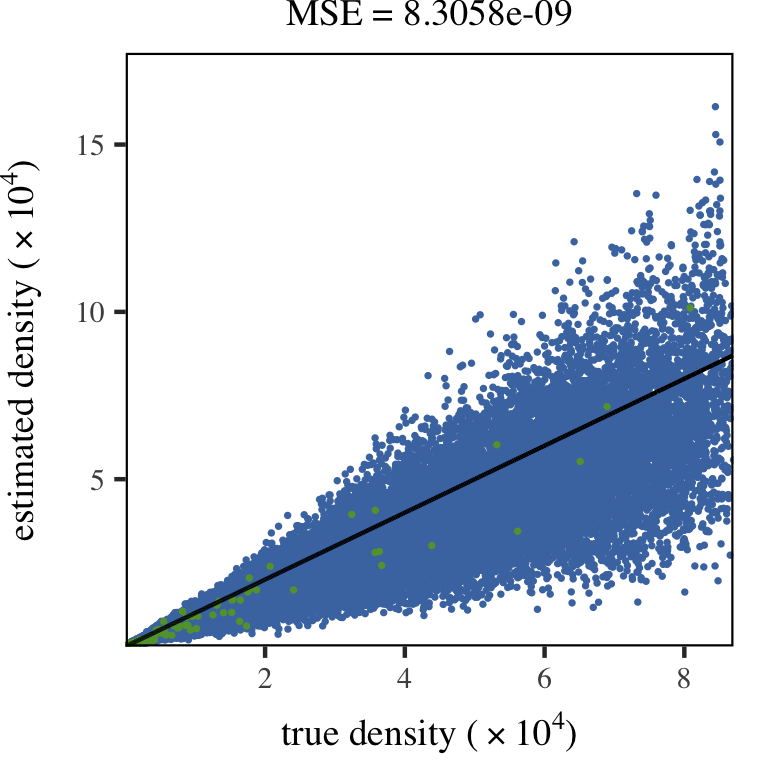
\includegraphics[keepaspectratio=true, width=\textwidth, height=0.23\textheight]{result/img/results_ferdosi_1_60000_mbe_silverman}
	\caption{Set \ferdosiOne, \mbe}
	\label{fig:results:singlesphere:mbe:ferdosi1}
\end{subfigure}
% Ferdosi 1 - SAMBE
\begin{subfigure}{0.3\textwidth}
	\centering
	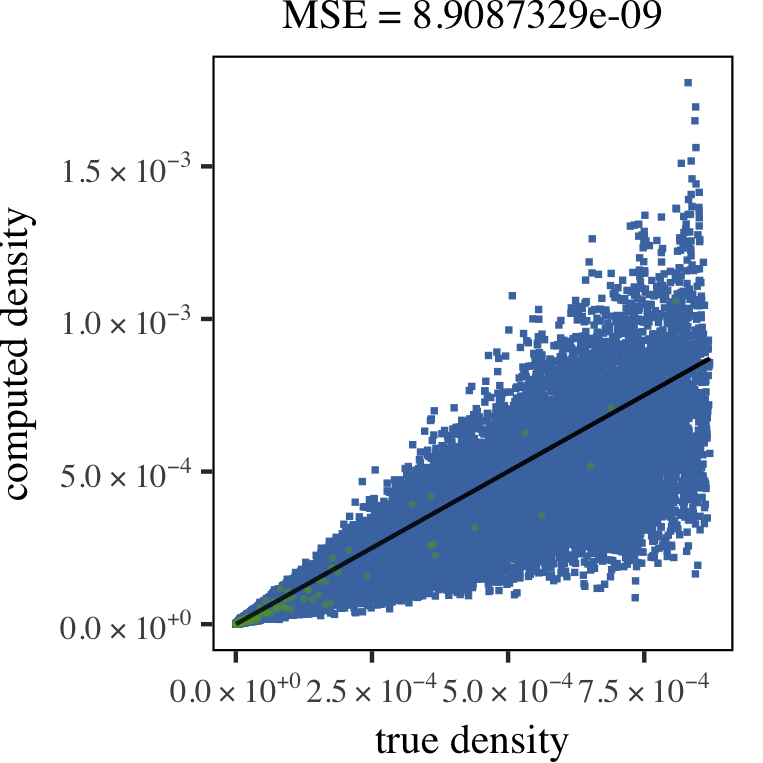
\includegraphics[keepaspectratio=true, width=\textwidth, height=0.23\textheight]{result/img/results_ferdosi_1_60000_sambe_silverman}
	\caption{Set \ferdosiOne, \sambe}
	\label{fig:results:singlesphere:sambe:ferdosi1}
\end{subfigure}
\subfigvspace
% Baakman 1	- MBE
\begin{subfigure}{0.3\textwidth}
	\centering
	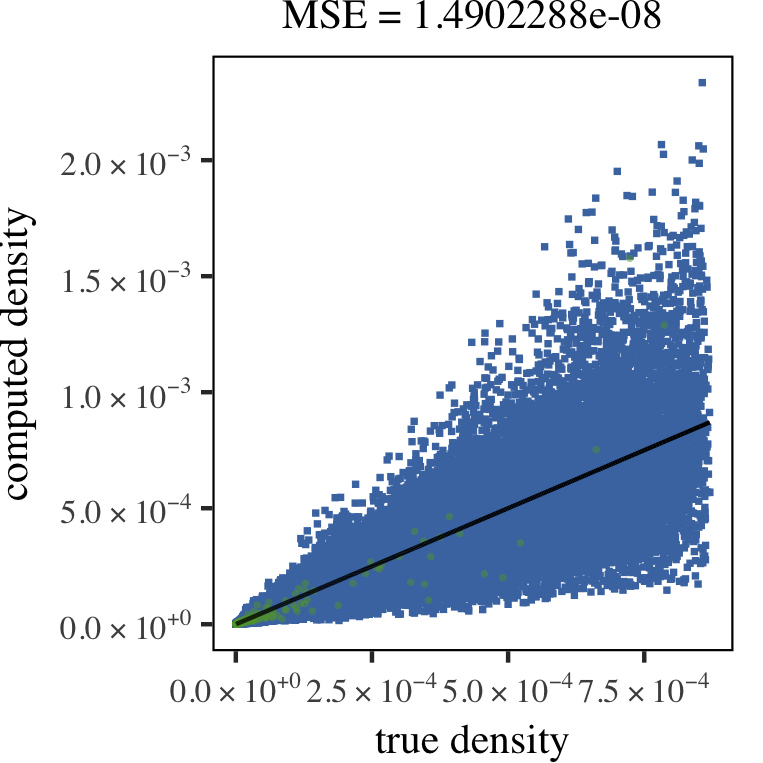
\includegraphics[keepaspectratio=true, width=\textwidth, height=0.23\textheight]{result/img/results_baakman_1_60000_mbe_silverman}
	\caption{Set \baakmanOne, \mbe}
	\label{fig:results:singlesphere:mbe:baakman1}
\end{subfigure}
% Baakman 1	- SAMBE
\begin{subfigure}{0.3\textwidth}
	\centering
	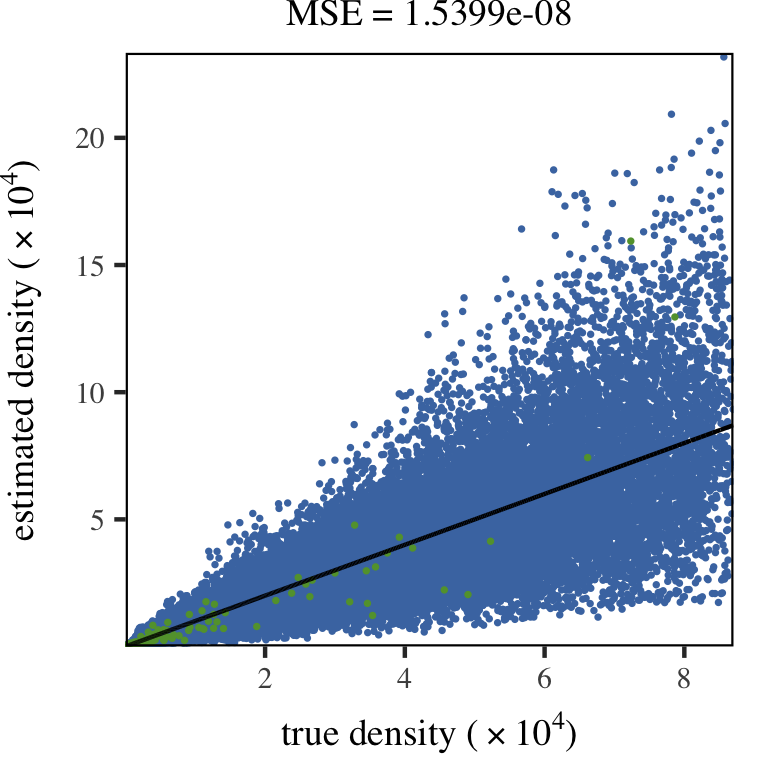
\includegraphics[keepaspectratio=true, width=\textwidth, height=0.23\textheight]{result/img/results_baakman_1_60000_sambe_silverman}
	\caption{Set \baakmanOne, \sambe}
	\label{fig:results:singlesphere:sambe:baakman1}
\end{subfigure}
\subfigvspace
% Baakman 4 - MBE
\begin{subfigure}{0.3\textwidth}
	\centering
	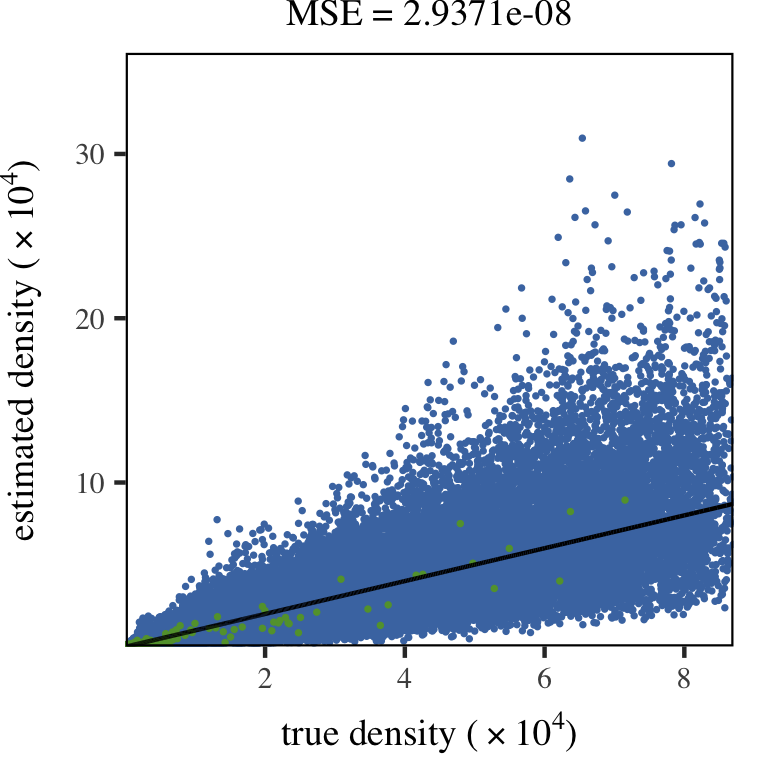
\includegraphics[keepaspectratio=true, width=\textwidth, height=0.23\textheight]{result/img/results_baakman_4_60000_mbe_silverman}
	\caption{Set \baakmanFour, \mbe}
	\label{fig:results:singlesphere:mbe:baakman4}
\end{subfigure}	
% Baakman 4 - SAMBE
\begin{subfigure}{0.3\textwidth}
	\centering
	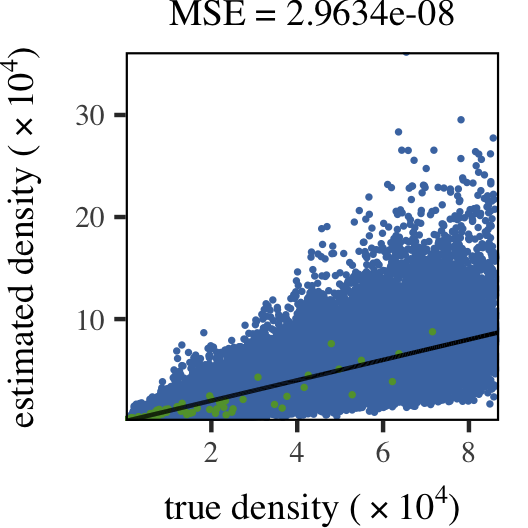
\includegraphics[keepaspectratio=true, width=\textwidth, height=0.23\textheight]{result/img/results_baakman_4_60000_sambe_silverman}
	\caption{Set \baakmanFour, \sambe}
	\label{fig:results:singlesphere:sambe:baakman4}
\end{subfigure}		
\subfigvspace
% Baakman 5 - MBE
\begin{subfigure}{0.3\textwidth}
	\centering
	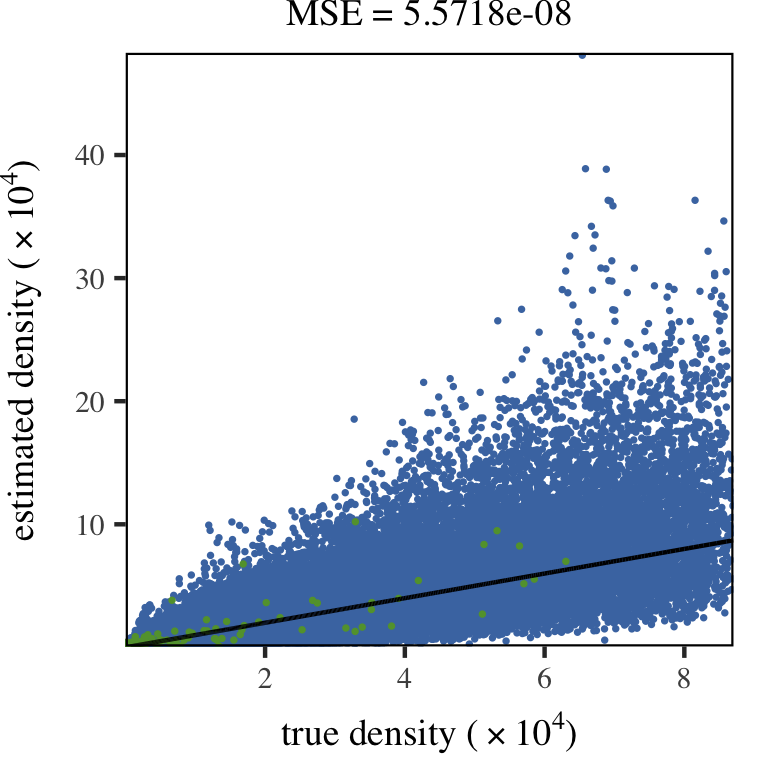
\includegraphics[keepaspectratio=true, width=\textwidth, height=0.23\textheight]{result/img/results_baakman_5_60000_mbe_silverman}
	\caption{Set \baakmanFive, \mbe}
	\label{fig:results:singlesphere:mbe:baakman5}
\end{subfigure}
% Baakman 5 - SAMBE
\begin{subfigure}{0.3\textwidth}
	\centering
	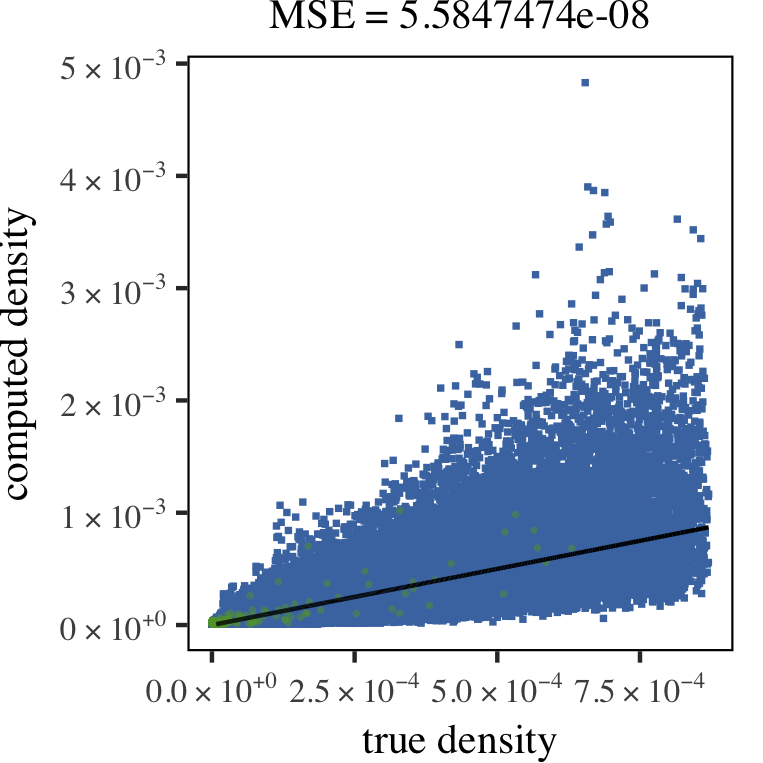
\includegraphics[keepaspectratio=true, width=\textwidth, height=0.23\textheight]{result/img/results_baakman_5_60000_sambe_silverman}
	\caption{Set \baakmanFive, \sambe}
	\label{fig:results:singlesphere:sambe:baakman5}
\end{subfigure}	
		\caption{The density as estimated by \mbe and \sambe as a function of the known density of data sets \ferdosiOne through \baakmanFive.}
		\label{fig:results:singleSphere:comparativePlots}
	\end{figure*}
	%
	This is confirmed by the visualization of the results in \cref{fig:results:singleSphere:comparativePlots} where hardly any difference is visible between \cref{fig:results:singlesphere:mbe:ferdosi1,fig:results:singlesphere:mbe:baakman1,fig:results:singlesphere:mbe:baakman4,fig:results:singlesphere:mbe:baakman5}, and \cref{fig:results:singlesphere:sambe:ferdosi1,fig:results:singlesphere:sambe:baakman1,fig:results:singlesphere:sambe:baakman4,fig:results:singlesphere:sambe:baakman5}, respectively.
		%Ferdosi 1
		Comparing the plots associated with data set \ferdosiOne, we find that the shape-adaptive estimator tends to overestimate densities more than the symmetric estimator if the Gaussian component is spherical.
		% Baakman 4
		Based on \cref{fig:results:singlesphere:mbe:baakman4,fig:results:singlesphere:sambe:baakman4} the same holds for set \baakmanFour.
	% Focus on components
	Comparing the performance within data sets between the two components showed no marked differences between the estimators between components.

%ANISOTROPY
	\begin{table}
		\centering
		%!TEX root = ../../paper.tex

% \sisetup{
% 	table-format=1.3e+1,
% 	scientific-notation=true, 
% 	table-number-alignment=center,
% }

% Mean and SD in single column
% \begin{tabular}{@{}c*{6}{c}@{}}
% \toprule
% ~				& Full Set 												& \legendComponentOne Gaussian 1						& \legendComponentTwo Gaussian 2						& \legendComponentThree Gaussian 3						& \legendComponentFour Gaussian 4					 	&  \legendComponentNoise Noise\\
% \midrule
% %
% \ferdosiTwo		& \meanSD{1.504005042371507e+00}{5.309582791641542e-01} & \meanSD{1.320121582169093e+00}{1.749869852989719e-01} & \meanSD{1.304784013773833e+00}{1.427734068384871e-01} & ~ 													& ~ 													& \meanSD{1.890276960903559e+00}{7.587403345342156e-01}\\
% \baakmanTwo 	& \meanSD{1.614716145373154e+00}{5.702499690627806e-01} & \meanSD{1.407377455694081e+00}{2.782480127488867e-01} & \meanSD{1.491043432778090e+00}{3.453168397321122e-01}	& ~ 													& ~ 													& \meanSD{11.948464282370670e+00}{7.826307984091438e-01}\\
% \ferdosiThree	& \meanSD{1.460357930082488e+00}{5.507084955708148e-01} & \meanSD{1.294023549845817e+00}{1.889517285607608e-01} & \meanSD{1.265946347671562e+00}{1.301150512342848e-01} & \meanSD{1.291829938425150e+00}{2.103396722315814e-01} & \meanSD{1.275739356043035e+00}{1.654855348814119e-01} & \meanSD{1.819950324176552e+00}{8.111641695146756e-01} \\
% \baakmanThree 	& \meanSD{1.532493079967588e+00}{5.713672219810757e-01} & \meanSD{1.314980484677339e+00}{2.190657831683435e-01} & \meanSD{1.487242917765238e+00}{3.393090417977690e-01} & \meanSD{1.291829938425150e+00}{2.103396722315814e-01} & \meanSD{1.396015162355687e+00}{2.851380764085146e-01} & \meanSD{1.854880861700560e+00}{8.195085323228068e-01}\\
% %
% \bottomrule
% \end{tabular}

\small
\sisetup{
	table-format=1.4,
	scientific-notation=fixed,
	table-number-alignment=center,
	fixed-exponent=0,
	round-mode=figures,
	round-precision=4
}


\begin{tabular}{@{}c*{12}{S}@{}}
\toprule
 				& \multicolumn{2}{c}{~} 						& \multicolumn{2}{c}{\legendComponentOne Gaussian 1} 	& \multicolumn{2}{c}{\legendComponentTwo Gaussian 2}	& \multicolumn{2}{c}{\legendComponentThree Gaussian 3}	& \multicolumn{2}{c}{\legendComponentFour Gaussian 4}	& \multicolumn{2}{c}{\legendComponentNoise Noise} \\
															  	\cmidrule(lr){4-5}							  				\cmidrule(lr){6-7}							  			\cmidrule(lr){8-9} 							  			\cmidrule(lr){10-11} 							  \cmidrule(lr){12-13}
~				& {\mean}				& {\SD}			& {\mean}				 & {\SD}			& {\mean}				 & {\SD}			 & {\mean}				& {\SD}			& {\mean}				& {\SD}			& {\mean}					& {\SD}\\ 			
\midrule
\ferdosiTwo		& 1.504005042371507e+00 & 5.309582791641542e-01 & 1.320121582169093e+00 & 1.749869852989719e-01 & 1.304784013773833e+00 & 1.427734068384871e-01 &  						&  						& 	 					&  							& 1.890276960903559e+00 	& 7.587403345342156e-01\\
\baakmanTwo 	& 1.614716145373154e+00 & 5.702499690627806e-01 & 1.407377455694081e+00 & 2.782480127488867e-01 & 1.491043432778090e+00 & 3.453168397321122e-01 &  						&  						& 	 					&  							& 1.948464282370670e+00 	& 7.826307984091438e-01\\
\ferdosiThree 	& 1.460357930082488e+00 & 5.507084955708148e-01 & 1.294023549845817e+00 & 1.889517285607608e-01 & 1.265946347671562e+00 & 1.301150512342848e-01 & 1.291829938425150e+00 & 2.103396722315814e-01 & 1.275739356043035e+00 & 1.654855348814119e-01 	& 1.819950324176552e+00 	& 8.111641695146756e-01 \\
\baakmanThree 	& 1.532493079967588e+00 & 5.713672219810757e-01 & 1.314980484677339e+00 & 2.190657831683435e-01 & 1.487242917765238e+00 & 3.393090417977690e-01 & 1.291829938425150e+00 & 2.103396722315814e-01 & 1.396015162355687e+00 & 2.851380764085146e-01 	& 1.854880861700560e+00 	& 8.195085323228068e-01\\
\bottomrule
\end{tabular}
		\caption{The mean (\mean) and the standard deviation (\SD) of the anisotropy of the kernels used for the data sets with a single Gaussian.}
		\label{tab:results:singleSphere:anisotropy}
	\end{table}
	%
	% General
	\Cref{tab:results:singleSphere:anisotropy} presents the mean and the standard deviation of the anisotropy of the kernels used for the different data sets. Comparing the means we find a positive correlation between the anisotropy of the Gaussian component of the data set and the mean anisotropy of the kernels. The same positive correlation can be observed for the standard deviation. Furthermore as the anisotropy of the Gaussian component increases, the anisotropy of the kernels associated with points sampled from the uniform random background rises.
	% Focus on components
	Reviewing these statistics of the components of the data sets reveals that the increase in average anisotropy is primarily caused by an increase in anisotropy of kernels of points sampled from the Gaussian component. The mean anisotropy of the background component stays relatively constant. Furthermore as the Gaussian component is more anisotropic the variation in anisotropy of the kernels increases.

%Summary
To summarize; in spite of differences in anisotropy of the used kernels we have observed very few differences between the two estimators. Using shape-adaptive kernels did not yield the expected gain in performance. We did find the hypothesized influence of the anisotropy of the Gaussian components on the shape of the kernels. Furthermore the kernels associated with points sampled from the background are more anisotropic than those belonging to points drawn from the Gaussian distribution.


\section{Results}
\label{s:results}
%!TEX root = ../../paper.tex

This section compares the performance of the Modified Breiman Estimator with symmetric and shape-adaptive kernels on data sets that contain one Gaussian component.
%MSE
	\begin{table}
		\centering
		%!TEX root = ../../paper.tex

\begin{tabular}{l*{2}{S[scientific-notation=true, round-mode=places,round-precision=3]}}
\toprule
~ 				& \multicolumn{2}{c}{Estimator}\\ \cmidrule{2-3}
Set				& {\mbe}					& {\sambe}	\\
\midrule
\ferdosiOne		& 8.30580618349064E-09		&  8.9087329457441E-09 \\
\baakmanOne		& 1.49022877061299E-08		&  1.5398737157543E-08 \\	
\baakmanFour	& 2.93709420107411E-08		&  2.9634323205557E-08 \\	
\baakmanFive	& 5.57179476550916E-08		&  5.5847473903432E-08 \\	
\bottomrule
\end{tabular}
		\caption{\Mses of the estimator with fixed-shape (\mbe) and shape-adaptive (\sambe) kernels on data set \ferdosiOne through \baakmanFive.}
		\label{tab:results:singleSphere:mse}
	\end{table}
	%
	Comparing the \mses of the \mbe with those of \sambe in \cref{tab:results:singleSphere:mse} we find that the estimators perform comparably, but that the fixed-shape estimator consistently gives a slightly lower \mse.

%PLOTS
	\begin{figure*}
		\centering
		%!TEX root = ../../paper.tex

% Ferdosi 1 - MBE
\begin{subfigure}{0.3\textwidth}
	\centering
	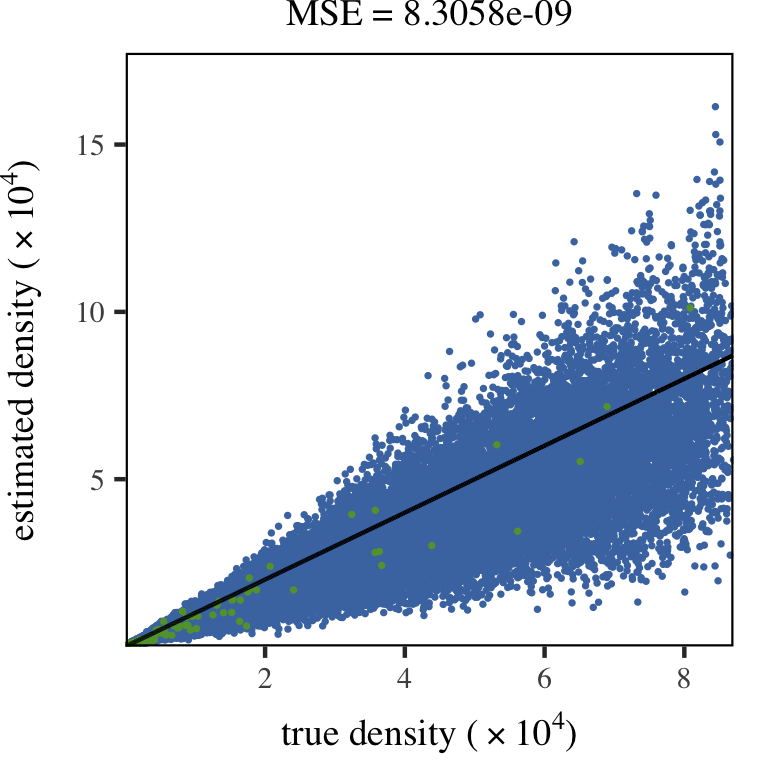
\includegraphics[keepaspectratio=true, width=\textwidth, height=0.23\textheight]{result/img/results_ferdosi_1_60000_mbe_silverman}
	\caption{Set \ferdosiOne, \mbe}
	\label{fig:results:singlesphere:mbe:ferdosi1}
\end{subfigure}
% Ferdosi 1 - SAMBE
\begin{subfigure}{0.3\textwidth}
	\centering
	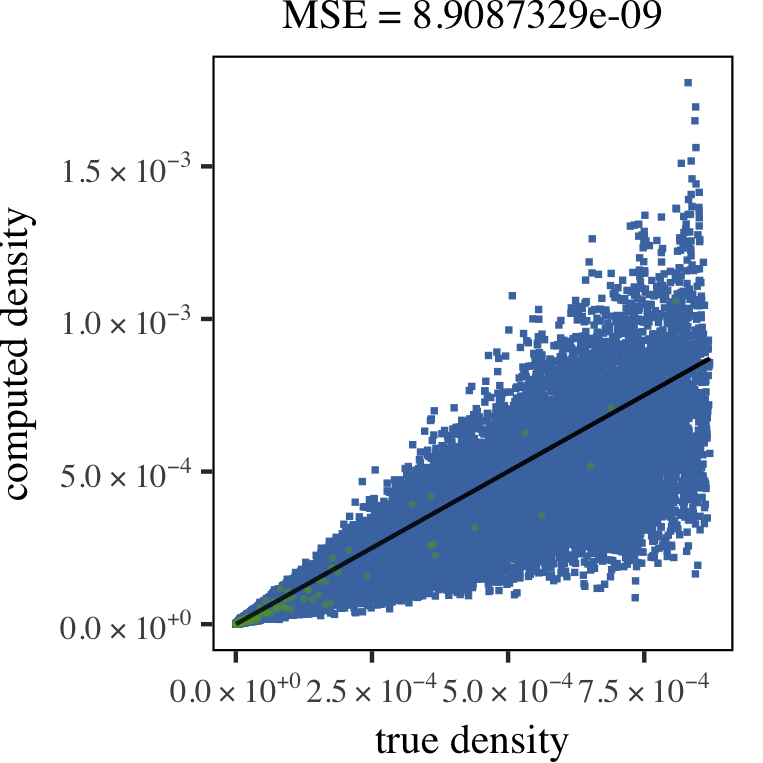
\includegraphics[keepaspectratio=true, width=\textwidth, height=0.23\textheight]{result/img/results_ferdosi_1_60000_sambe_silverman}
	\caption{Set \ferdosiOne, \sambe}
	\label{fig:results:singlesphere:sambe:ferdosi1}
\end{subfigure}
\subfigvspace
% Baakman 1	- MBE
\begin{subfigure}{0.3\textwidth}
	\centering
	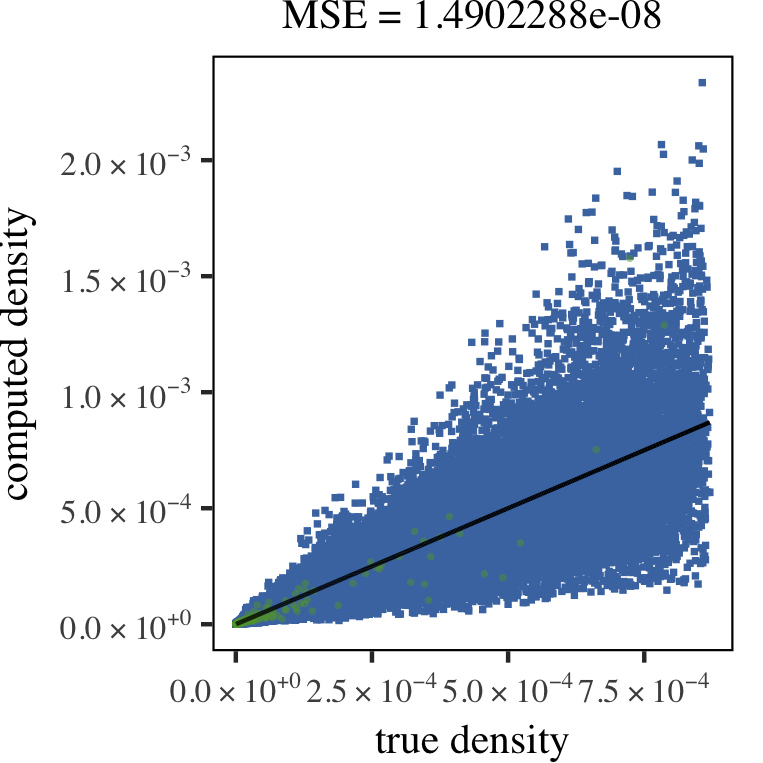
\includegraphics[keepaspectratio=true, width=\textwidth, height=0.23\textheight]{result/img/results_baakman_1_60000_mbe_silverman}
	\caption{Set \baakmanOne, \mbe}
	\label{fig:results:singlesphere:mbe:baakman1}
\end{subfigure}
% Baakman 1	- SAMBE
\begin{subfigure}{0.3\textwidth}
	\centering
	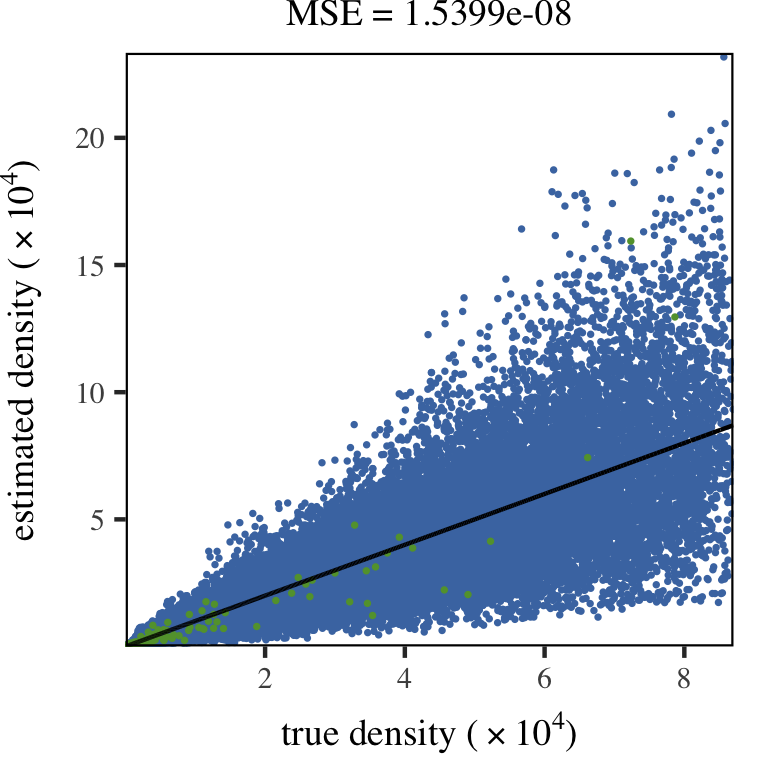
\includegraphics[keepaspectratio=true, width=\textwidth, height=0.23\textheight]{result/img/results_baakman_1_60000_sambe_silverman}
	\caption{Set \baakmanOne, \sambe}
	\label{fig:results:singlesphere:sambe:baakman1}
\end{subfigure}
\subfigvspace
% Baakman 4 - MBE
\begin{subfigure}{0.3\textwidth}
	\centering
	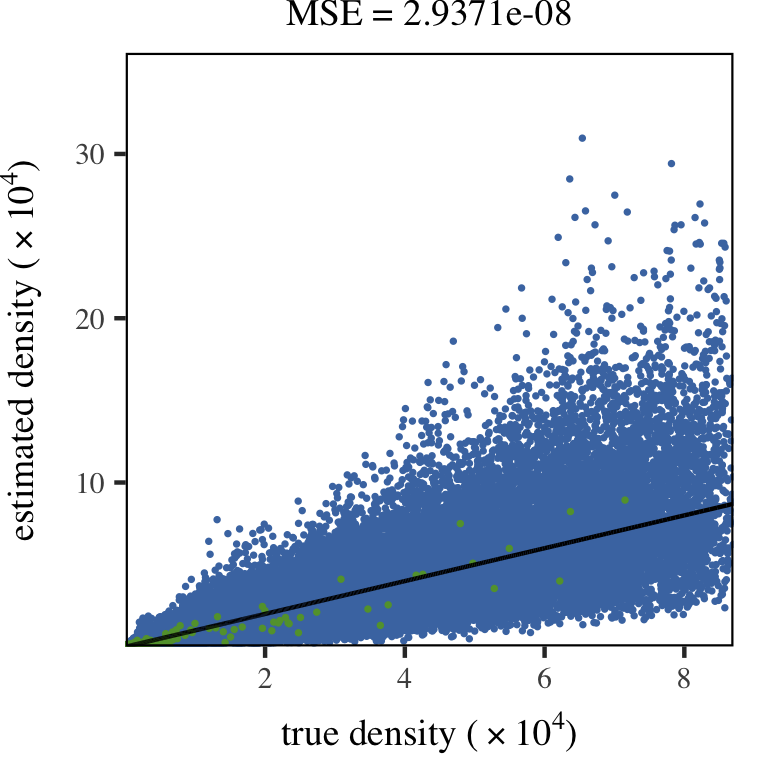
\includegraphics[keepaspectratio=true, width=\textwidth, height=0.23\textheight]{result/img/results_baakman_4_60000_mbe_silverman}
	\caption{Set \baakmanFour, \mbe}
	\label{fig:results:singlesphere:mbe:baakman4}
\end{subfigure}	
% Baakman 4 - SAMBE
\begin{subfigure}{0.3\textwidth}
	\centering
	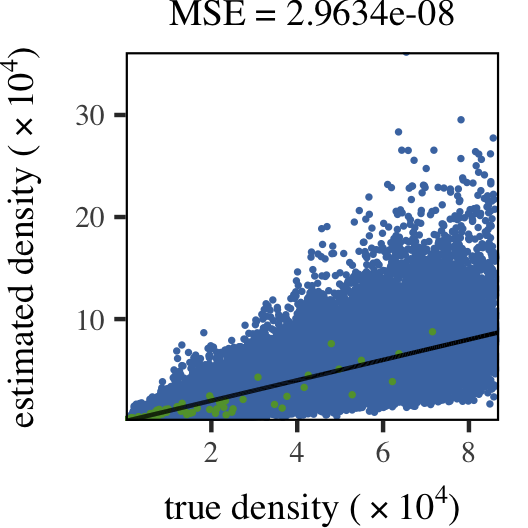
\includegraphics[keepaspectratio=true, width=\textwidth, height=0.23\textheight]{result/img/results_baakman_4_60000_sambe_silverman}
	\caption{Set \baakmanFour, \sambe}
	\label{fig:results:singlesphere:sambe:baakman4}
\end{subfigure}		
\subfigvspace
% Baakman 5 - MBE
\begin{subfigure}{0.3\textwidth}
	\centering
	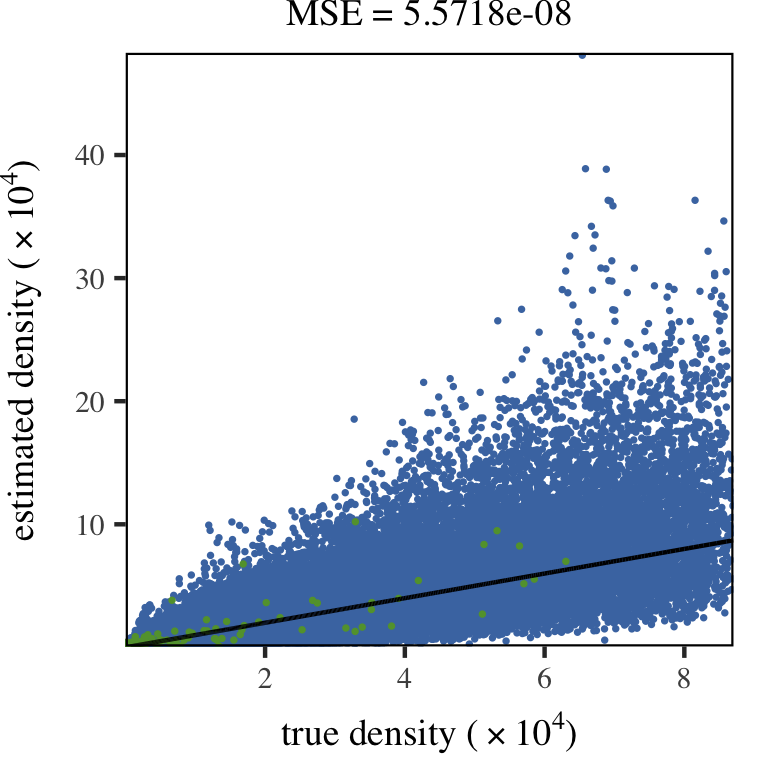
\includegraphics[keepaspectratio=true, width=\textwidth, height=0.23\textheight]{result/img/results_baakman_5_60000_mbe_silverman}
	\caption{Set \baakmanFive, \mbe}
	\label{fig:results:singlesphere:mbe:baakman5}
\end{subfigure}
% Baakman 5 - SAMBE
\begin{subfigure}{0.3\textwidth}
	\centering
	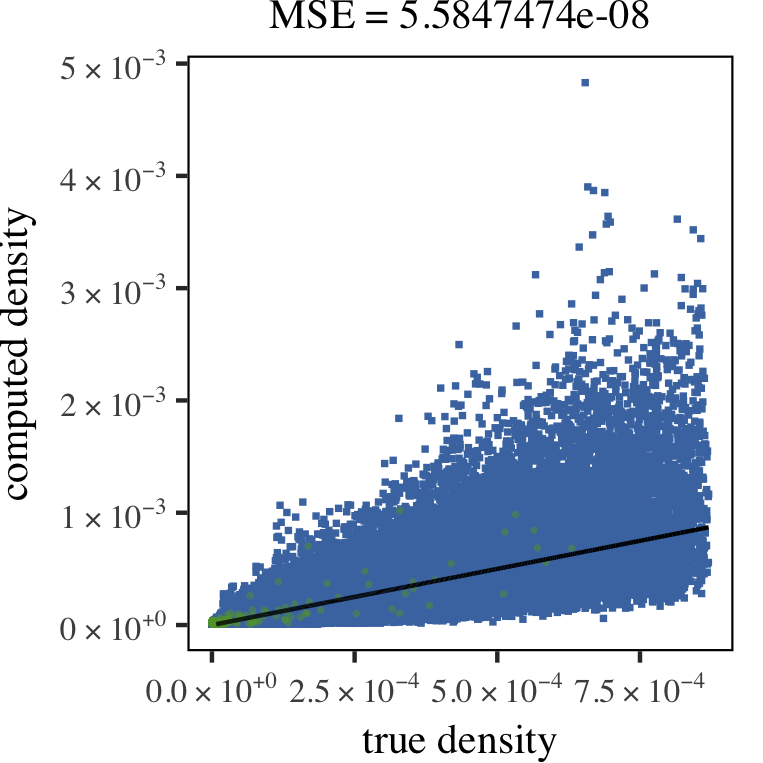
\includegraphics[keepaspectratio=true, width=\textwidth, height=0.23\textheight]{result/img/results_baakman_5_60000_sambe_silverman}
	\caption{Set \baakmanFive, \sambe}
	\label{fig:results:singlesphere:sambe:baakman5}
\end{subfigure}	
		\caption{The density as estimated by \mbe and \sambe as a function of the known density of data sets \ferdosiOne through \baakmanFive.}
		\label{fig:results:singleSphere:comparativePlots}
	\end{figure*}
	%
	This is confirmed by the visualization of the results in \cref{fig:results:singleSphere:comparativePlots} where hardly any difference is visible between \cref{fig:results:singlesphere:mbe:ferdosi1,fig:results:singlesphere:mbe:baakman1,fig:results:singlesphere:mbe:baakman4,fig:results:singlesphere:mbe:baakman5}, and \cref{fig:results:singlesphere:sambe:ferdosi1,fig:results:singlesphere:sambe:baakman1,fig:results:singlesphere:sambe:baakman4,fig:results:singlesphere:sambe:baakman5}, respectively.
		%Ferdosi 1
		Comparing the plots associated with data set \ferdosiOne, we find that the shape-adaptive estimator tends to overestimate densities more than the symmetric estimator if the Gaussian component is spherical.
		% Baakman 4
		Based on \cref{fig:results:singlesphere:mbe:baakman4,fig:results:singlesphere:sambe:baakman4} the same holds for set \baakmanFour.
	% Focus on components
	Comparing the performance within data sets between the two components showed no marked differences between the estimators between components.

%ANISOTROPY
	\begin{table}
		\centering
		%!TEX root = ../../paper.tex

% \sisetup{
% 	table-format=1.3e+1,
% 	scientific-notation=true, 
% 	table-number-alignment=center,
% }

% Mean and SD in single column
% \begin{tabular}{@{}c*{6}{c}@{}}
% \toprule
% ~				& Full Set 												& \legendComponentOne Gaussian 1						& \legendComponentTwo Gaussian 2						& \legendComponentThree Gaussian 3						& \legendComponentFour Gaussian 4					 	&  \legendComponentNoise Noise\\
% \midrule
% %
% \ferdosiTwo		& \meanSD{1.504005042371507e+00}{5.309582791641542e-01} & \meanSD{1.320121582169093e+00}{1.749869852989719e-01} & \meanSD{1.304784013773833e+00}{1.427734068384871e-01} & ~ 													& ~ 													& \meanSD{1.890276960903559e+00}{7.587403345342156e-01}\\
% \baakmanTwo 	& \meanSD{1.614716145373154e+00}{5.702499690627806e-01} & \meanSD{1.407377455694081e+00}{2.782480127488867e-01} & \meanSD{1.491043432778090e+00}{3.453168397321122e-01}	& ~ 													& ~ 													& \meanSD{11.948464282370670e+00}{7.826307984091438e-01}\\
% \ferdosiThree	& \meanSD{1.460357930082488e+00}{5.507084955708148e-01} & \meanSD{1.294023549845817e+00}{1.889517285607608e-01} & \meanSD{1.265946347671562e+00}{1.301150512342848e-01} & \meanSD{1.291829938425150e+00}{2.103396722315814e-01} & \meanSD{1.275739356043035e+00}{1.654855348814119e-01} & \meanSD{1.819950324176552e+00}{8.111641695146756e-01} \\
% \baakmanThree 	& \meanSD{1.532493079967588e+00}{5.713672219810757e-01} & \meanSD{1.314980484677339e+00}{2.190657831683435e-01} & \meanSD{1.487242917765238e+00}{3.393090417977690e-01} & \meanSD{1.291829938425150e+00}{2.103396722315814e-01} & \meanSD{1.396015162355687e+00}{2.851380764085146e-01} & \meanSD{1.854880861700560e+00}{8.195085323228068e-01}\\
% %
% \bottomrule
% \end{tabular}

\small
\sisetup{
	table-format=1.4,
	scientific-notation=fixed,
	table-number-alignment=center,
	fixed-exponent=0,
	round-mode=figures,
	round-precision=4
}


\begin{tabular}{@{}c*{12}{S}@{}}
\toprule
 				& \multicolumn{2}{c}{~} 						& \multicolumn{2}{c}{\legendComponentOne Gaussian 1} 	& \multicolumn{2}{c}{\legendComponentTwo Gaussian 2}	& \multicolumn{2}{c}{\legendComponentThree Gaussian 3}	& \multicolumn{2}{c}{\legendComponentFour Gaussian 4}	& \multicolumn{2}{c}{\legendComponentNoise Noise} \\
															  	\cmidrule(lr){4-5}							  				\cmidrule(lr){6-7}							  			\cmidrule(lr){8-9} 							  			\cmidrule(lr){10-11} 							  \cmidrule(lr){12-13}
~				& {\mean}				& {\SD}			& {\mean}				 & {\SD}			& {\mean}				 & {\SD}			 & {\mean}				& {\SD}			& {\mean}				& {\SD}			& {\mean}					& {\SD}\\ 			
\midrule
\ferdosiTwo		& 1.504005042371507e+00 & 5.309582791641542e-01 & 1.320121582169093e+00 & 1.749869852989719e-01 & 1.304784013773833e+00 & 1.427734068384871e-01 &  						&  						& 	 					&  							& 1.890276960903559e+00 	& 7.587403345342156e-01\\
\baakmanTwo 	& 1.614716145373154e+00 & 5.702499690627806e-01 & 1.407377455694081e+00 & 2.782480127488867e-01 & 1.491043432778090e+00 & 3.453168397321122e-01 &  						&  						& 	 					&  							& 1.948464282370670e+00 	& 7.826307984091438e-01\\
\ferdosiThree 	& 1.460357930082488e+00 & 5.507084955708148e-01 & 1.294023549845817e+00 & 1.889517285607608e-01 & 1.265946347671562e+00 & 1.301150512342848e-01 & 1.291829938425150e+00 & 2.103396722315814e-01 & 1.275739356043035e+00 & 1.654855348814119e-01 	& 1.819950324176552e+00 	& 8.111641695146756e-01 \\
\baakmanThree 	& 1.532493079967588e+00 & 5.713672219810757e-01 & 1.314980484677339e+00 & 2.190657831683435e-01 & 1.487242917765238e+00 & 3.393090417977690e-01 & 1.291829938425150e+00 & 2.103396722315814e-01 & 1.396015162355687e+00 & 2.851380764085146e-01 	& 1.854880861700560e+00 	& 8.195085323228068e-01\\
\bottomrule
\end{tabular}
		\caption{The mean (\mean) and the standard deviation (\SD) of the anisotropy of the kernels used for the data sets with a single Gaussian.}
		\label{tab:results:singleSphere:anisotropy}
	\end{table}
	%
	% General
	\Cref{tab:results:singleSphere:anisotropy} presents the mean and the standard deviation of the anisotropy of the kernels used for the different data sets. Comparing the means we find a positive correlation between the anisotropy of the Gaussian component of the data set and the mean anisotropy of the kernels. The same positive correlation can be observed for the standard deviation. Furthermore as the anisotropy of the Gaussian component increases, the anisotropy of the kernels associated with points sampled from the uniform random background rises.
	% Focus on components
	Reviewing these statistics of the components of the data sets reveals that the increase in average anisotropy is primarily caused by an increase in anisotropy of kernels of points sampled from the Gaussian component. The mean anisotropy of the background component stays relatively constant. Furthermore as the Gaussian component is more anisotropic the variation in anisotropy of the kernels increases.

%Summary
To summarize; in spite of differences in anisotropy of the used kernels we have observed very few differences between the two estimators. Using shape-adaptive kernels did not yield the expected gain in performance. We did find the hypothesized influence of the anisotropy of the Gaussian components on the shape of the kernels. Furthermore the kernels associated with points sampled from the background are more anisotropic than those belonging to points drawn from the Gaussian distribution.


\section{Discussion}
\label{s:discussion}
%!TEX root = ../../paper.tex

This section compares the performance of the Modified Breiman Estimator with symmetric and shape-adaptive kernels on data sets that contain one Gaussian component.
%MSE
	\begin{table}
		\centering
		%!TEX root = ../../paper.tex

\begin{tabular}{l*{2}{S[scientific-notation=true, round-mode=places,round-precision=3]}}
\toprule
~ 				& \multicolumn{2}{c}{Estimator}\\ \cmidrule{2-3}
Set				& {\mbe}					& {\sambe}	\\
\midrule
\ferdosiOne		& 8.30580618349064E-09		&  8.9087329457441E-09 \\
\baakmanOne		& 1.49022877061299E-08		&  1.5398737157543E-08 \\	
\baakmanFour	& 2.93709420107411E-08		&  2.9634323205557E-08 \\	
\baakmanFive	& 5.57179476550916E-08		&  5.5847473903432E-08 \\	
\bottomrule
\end{tabular}
		\caption{\Mses of the estimator with fixed-shape (\mbe) and shape-adaptive (\sambe) kernels on data set \ferdosiOne through \baakmanFive.}
		\label{tab:results:singleSphere:mse}
	\end{table}
	%
	Comparing the \mses of the \mbe with those of \sambe in \cref{tab:results:singleSphere:mse} we find that the estimators perform comparably, but that the fixed-shape estimator consistently gives a slightly lower \mse.

%PLOTS
	\begin{figure*}
		\centering
		%!TEX root = ../../paper.tex

% Ferdosi 1 - MBE
\begin{subfigure}{0.3\textwidth}
	\centering
	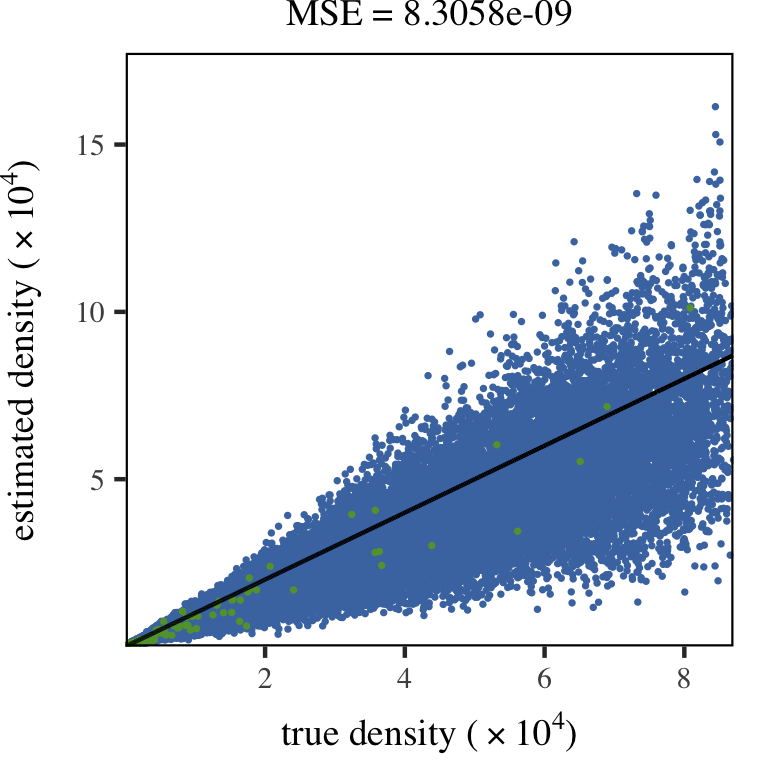
\includegraphics[keepaspectratio=true, width=\textwidth, height=0.23\textheight]{result/img/results_ferdosi_1_60000_mbe_silverman}
	\caption{Set \ferdosiOne, \mbe}
	\label{fig:results:singlesphere:mbe:ferdosi1}
\end{subfigure}
% Ferdosi 1 - SAMBE
\begin{subfigure}{0.3\textwidth}
	\centering
	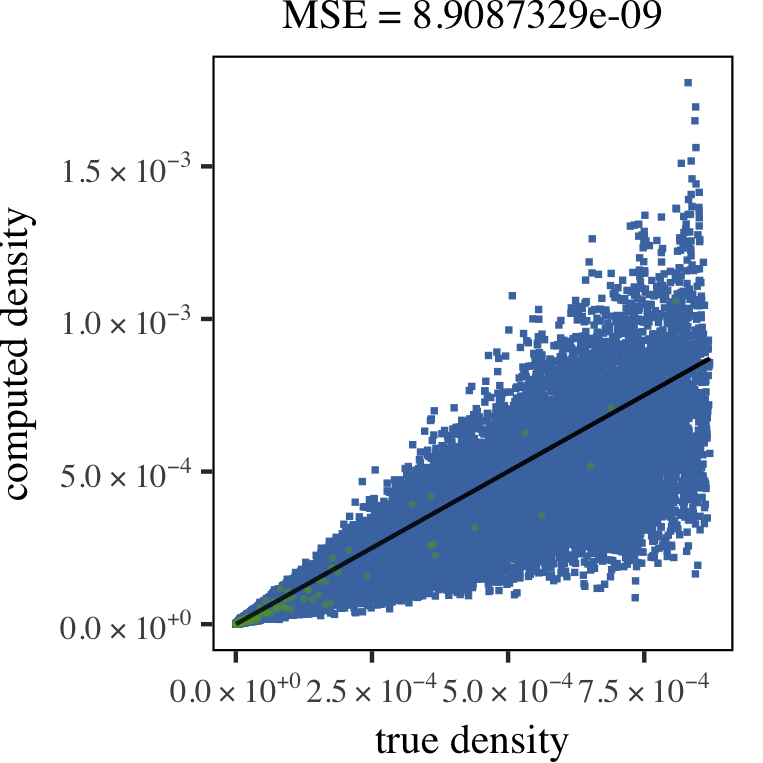
\includegraphics[keepaspectratio=true, width=\textwidth, height=0.23\textheight]{result/img/results_ferdosi_1_60000_sambe_silverman}
	\caption{Set \ferdosiOne, \sambe}
	\label{fig:results:singlesphere:sambe:ferdosi1}
\end{subfigure}
\subfigvspace
% Baakman 1	- MBE
\begin{subfigure}{0.3\textwidth}
	\centering
	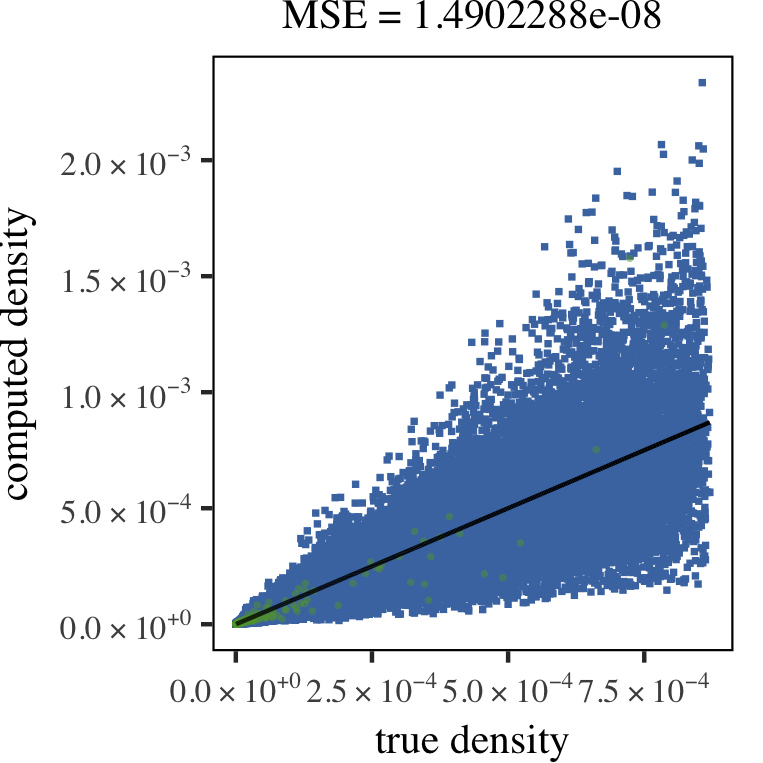
\includegraphics[keepaspectratio=true, width=\textwidth, height=0.23\textheight]{result/img/results_baakman_1_60000_mbe_silverman}
	\caption{Set \baakmanOne, \mbe}
	\label{fig:results:singlesphere:mbe:baakman1}
\end{subfigure}
% Baakman 1	- SAMBE
\begin{subfigure}{0.3\textwidth}
	\centering
	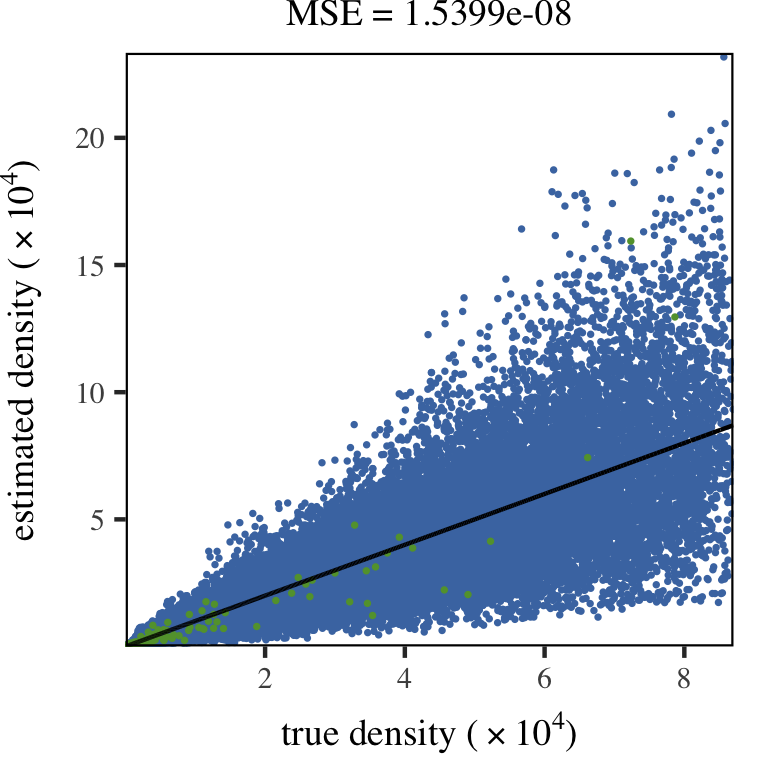
\includegraphics[keepaspectratio=true, width=\textwidth, height=0.23\textheight]{result/img/results_baakman_1_60000_sambe_silverman}
	\caption{Set \baakmanOne, \sambe}
	\label{fig:results:singlesphere:sambe:baakman1}
\end{subfigure}
\subfigvspace
% Baakman 4 - MBE
\begin{subfigure}{0.3\textwidth}
	\centering
	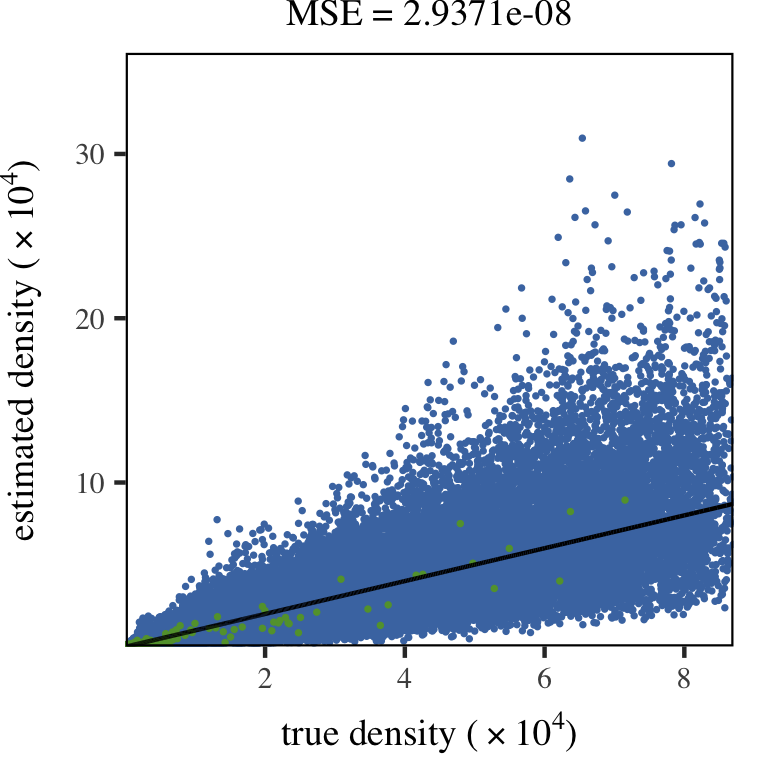
\includegraphics[keepaspectratio=true, width=\textwidth, height=0.23\textheight]{result/img/results_baakman_4_60000_mbe_silverman}
	\caption{Set \baakmanFour, \mbe}
	\label{fig:results:singlesphere:mbe:baakman4}
\end{subfigure}	
% Baakman 4 - SAMBE
\begin{subfigure}{0.3\textwidth}
	\centering
	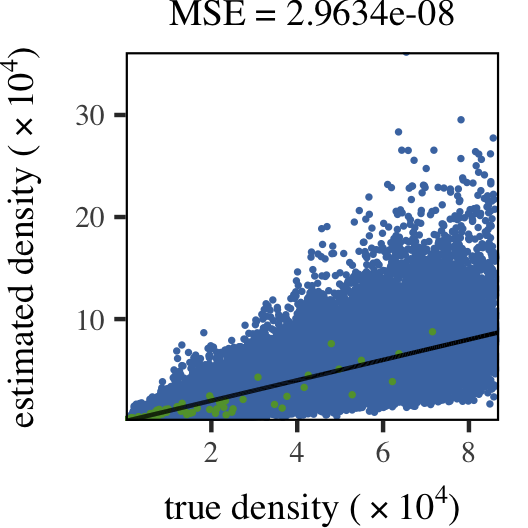
\includegraphics[keepaspectratio=true, width=\textwidth, height=0.23\textheight]{result/img/results_baakman_4_60000_sambe_silverman}
	\caption{Set \baakmanFour, \sambe}
	\label{fig:results:singlesphere:sambe:baakman4}
\end{subfigure}		
\subfigvspace
% Baakman 5 - MBE
\begin{subfigure}{0.3\textwidth}
	\centering
	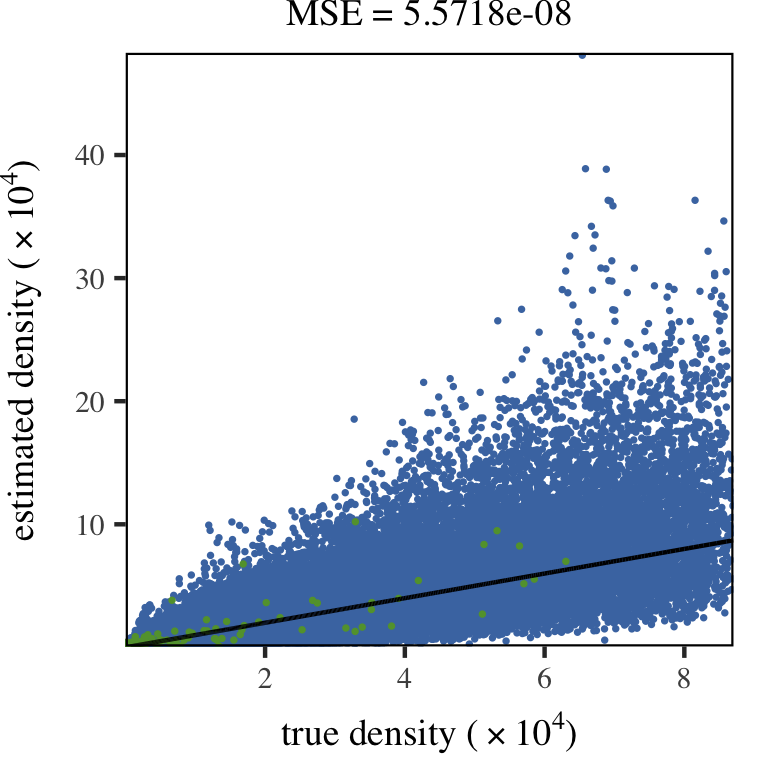
\includegraphics[keepaspectratio=true, width=\textwidth, height=0.23\textheight]{result/img/results_baakman_5_60000_mbe_silverman}
	\caption{Set \baakmanFive, \mbe}
	\label{fig:results:singlesphere:mbe:baakman5}
\end{subfigure}
% Baakman 5 - SAMBE
\begin{subfigure}{0.3\textwidth}
	\centering
	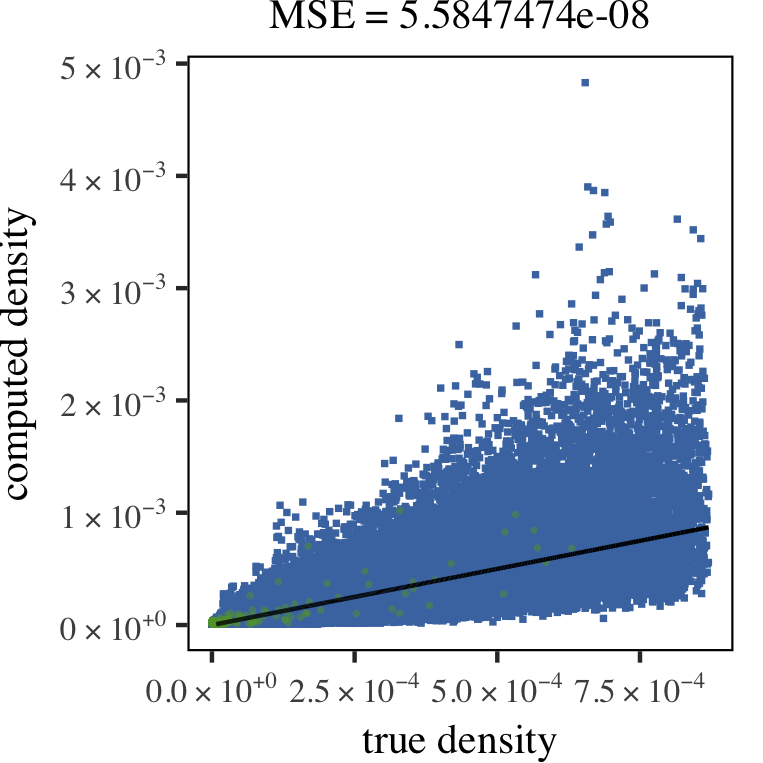
\includegraphics[keepaspectratio=true, width=\textwidth, height=0.23\textheight]{result/img/results_baakman_5_60000_sambe_silverman}
	\caption{Set \baakmanFive, \sambe}
	\label{fig:results:singlesphere:sambe:baakman5}
\end{subfigure}	
		\caption{The density as estimated by \mbe and \sambe as a function of the known density of data sets \ferdosiOne through \baakmanFive.}
		\label{fig:results:singleSphere:comparativePlots}
	\end{figure*}
	%
	This is confirmed by the visualization of the results in \cref{fig:results:singleSphere:comparativePlots} where hardly any difference is visible between \cref{fig:results:singlesphere:mbe:ferdosi1,fig:results:singlesphere:mbe:baakman1,fig:results:singlesphere:mbe:baakman4,fig:results:singlesphere:mbe:baakman5}, and \cref{fig:results:singlesphere:sambe:ferdosi1,fig:results:singlesphere:sambe:baakman1,fig:results:singlesphere:sambe:baakman4,fig:results:singlesphere:sambe:baakman5}, respectively.
		%Ferdosi 1
		Comparing the plots associated with data set \ferdosiOne, we find that the shape-adaptive estimator tends to overestimate densities more than the symmetric estimator if the Gaussian component is spherical.
		% Baakman 4
		Based on \cref{fig:results:singlesphere:mbe:baakman4,fig:results:singlesphere:sambe:baakman4} the same holds for set \baakmanFour.
	% Focus on components
	Comparing the performance within data sets between the two components showed no marked differences between the estimators between components.

%ANISOTROPY
	\begin{table}
		\centering
		%!TEX root = ../../paper.tex

% \sisetup{
% 	table-format=1.3e+1,
% 	scientific-notation=true, 
% 	table-number-alignment=center,
% }

% Mean and SD in single column
% \begin{tabular}{@{}c*{6}{c}@{}}
% \toprule
% ~				& Full Set 												& \legendComponentOne Gaussian 1						& \legendComponentTwo Gaussian 2						& \legendComponentThree Gaussian 3						& \legendComponentFour Gaussian 4					 	&  \legendComponentNoise Noise\\
% \midrule
% %
% \ferdosiTwo		& \meanSD{1.504005042371507e+00}{5.309582791641542e-01} & \meanSD{1.320121582169093e+00}{1.749869852989719e-01} & \meanSD{1.304784013773833e+00}{1.427734068384871e-01} & ~ 													& ~ 													& \meanSD{1.890276960903559e+00}{7.587403345342156e-01}\\
% \baakmanTwo 	& \meanSD{1.614716145373154e+00}{5.702499690627806e-01} & \meanSD{1.407377455694081e+00}{2.782480127488867e-01} & \meanSD{1.491043432778090e+00}{3.453168397321122e-01}	& ~ 													& ~ 													& \meanSD{11.948464282370670e+00}{7.826307984091438e-01}\\
% \ferdosiThree	& \meanSD{1.460357930082488e+00}{5.507084955708148e-01} & \meanSD{1.294023549845817e+00}{1.889517285607608e-01} & \meanSD{1.265946347671562e+00}{1.301150512342848e-01} & \meanSD{1.291829938425150e+00}{2.103396722315814e-01} & \meanSD{1.275739356043035e+00}{1.654855348814119e-01} & \meanSD{1.819950324176552e+00}{8.111641695146756e-01} \\
% \baakmanThree 	& \meanSD{1.532493079967588e+00}{5.713672219810757e-01} & \meanSD{1.314980484677339e+00}{2.190657831683435e-01} & \meanSD{1.487242917765238e+00}{3.393090417977690e-01} & \meanSD{1.291829938425150e+00}{2.103396722315814e-01} & \meanSD{1.396015162355687e+00}{2.851380764085146e-01} & \meanSD{1.854880861700560e+00}{8.195085323228068e-01}\\
% %
% \bottomrule
% \end{tabular}

\small
\sisetup{
	table-format=1.4,
	scientific-notation=fixed,
	table-number-alignment=center,
	fixed-exponent=0,
	round-mode=figures,
	round-precision=4
}


\begin{tabular}{@{}c*{12}{S}@{}}
\toprule
 				& \multicolumn{2}{c}{~} 						& \multicolumn{2}{c}{\legendComponentOne Gaussian 1} 	& \multicolumn{2}{c}{\legendComponentTwo Gaussian 2}	& \multicolumn{2}{c}{\legendComponentThree Gaussian 3}	& \multicolumn{2}{c}{\legendComponentFour Gaussian 4}	& \multicolumn{2}{c}{\legendComponentNoise Noise} \\
															  	\cmidrule(lr){4-5}							  				\cmidrule(lr){6-7}							  			\cmidrule(lr){8-9} 							  			\cmidrule(lr){10-11} 							  \cmidrule(lr){12-13}
~				& {\mean}				& {\SD}			& {\mean}				 & {\SD}			& {\mean}				 & {\SD}			 & {\mean}				& {\SD}			& {\mean}				& {\SD}			& {\mean}					& {\SD}\\ 			
\midrule
\ferdosiTwo		& 1.504005042371507e+00 & 5.309582791641542e-01 & 1.320121582169093e+00 & 1.749869852989719e-01 & 1.304784013773833e+00 & 1.427734068384871e-01 &  						&  						& 	 					&  							& 1.890276960903559e+00 	& 7.587403345342156e-01\\
\baakmanTwo 	& 1.614716145373154e+00 & 5.702499690627806e-01 & 1.407377455694081e+00 & 2.782480127488867e-01 & 1.491043432778090e+00 & 3.453168397321122e-01 &  						&  						& 	 					&  							& 1.948464282370670e+00 	& 7.826307984091438e-01\\
\ferdosiThree 	& 1.460357930082488e+00 & 5.507084955708148e-01 & 1.294023549845817e+00 & 1.889517285607608e-01 & 1.265946347671562e+00 & 1.301150512342848e-01 & 1.291829938425150e+00 & 2.103396722315814e-01 & 1.275739356043035e+00 & 1.654855348814119e-01 	& 1.819950324176552e+00 	& 8.111641695146756e-01 \\
\baakmanThree 	& 1.532493079967588e+00 & 5.713672219810757e-01 & 1.314980484677339e+00 & 2.190657831683435e-01 & 1.487242917765238e+00 & 3.393090417977690e-01 & 1.291829938425150e+00 & 2.103396722315814e-01 & 1.396015162355687e+00 & 2.851380764085146e-01 	& 1.854880861700560e+00 	& 8.195085323228068e-01\\
\bottomrule
\end{tabular}
		\caption{The mean (\mean) and the standard deviation (\SD) of the anisotropy of the kernels used for the data sets with a single Gaussian.}
		\label{tab:results:singleSphere:anisotropy}
	\end{table}
	%
	% General
	\Cref{tab:results:singleSphere:anisotropy} presents the mean and the standard deviation of the anisotropy of the kernels used for the different data sets. Comparing the means we find a positive correlation between the anisotropy of the Gaussian component of the data set and the mean anisotropy of the kernels. The same positive correlation can be observed for the standard deviation. Furthermore as the anisotropy of the Gaussian component increases, the anisotropy of the kernels associated with points sampled from the uniform random background rises.
	% Focus on components
	Reviewing these statistics of the components of the data sets reveals that the increase in average anisotropy is primarily caused by an increase in anisotropy of kernels of points sampled from the Gaussian component. The mean anisotropy of the background component stays relatively constant. Furthermore as the Gaussian component is more anisotropic the variation in anisotropy of the kernels increases.

%Summary
To summarize; in spite of differences in anisotropy of the used kernels we have observed very few differences between the two estimators. Using shape-adaptive kernels did not yield the expected gain in performance. We did find the hypothesized influence of the anisotropy of the Gaussian components on the shape of the kernels. Furthermore the kernels associated with points sampled from the background are more anisotropic than those belonging to points drawn from the Gaussian distribution.


\section{Conclusion}
\label{s:conclusion}
%!TEX root = paper.tex

We have found that the shape-adaptive Modified Breiman Estimator gives results comparable to those of the symmetric version of the estimator.
% Where SAMBE outperforms MBE
Anisotropic kernels have proven advantageous near the borders of the data sets. However this positive effect is negated by the number of points where the kernel is too isotropic, or too anisotropic for its local neighborhood. 
% Problems with SAMBE
	% High anisotropy of kernels in noise
	Kernels that are too anisotropic for their neighborhood occur mostly in the uniform random noise, due to the local neighborhood being sensitive to spurious, fine structures in the background, where the data is isotropic. 
	% High anistropy with high density
	Too isotropic kernels occur mostly with points near the mean of Gaussian components whose covariance matrix has a large eigensphere. 

% Further research
Both cases show that the estimator has problems with detecting the shape of the local neighborhood. One way of addressing this problem might be to (adaptively) increase the size of the local neighborhood. Another possible improvement could be to decide how anisotropic the kernel should be, based on its local neighborhood.

% Conclusion
In conclusion shape-adaptive kernels are a promising idea that definitely warrants the research needed to work out the kinks identified in this paper.


\printbibliography

\end{document}